\chapter{Wyniki eksperymentu}
\label{c5}

Dany rozdział zawiera wyniki z przeprowadzonych badań oraz wnioski. Każda aplikacja, która została napisana została przestawiona i opisana z różnych perspektyw. Na końcu rozdziału zostały przedstawione wady i zalety obu podejść. Z wyjątkiem ostatniej aplikacje zostały najpierw stworzone w App Inventorze, a następnie zostały przepisane na język Java.

\section{Aplikacje testujące wydajność}

\subsection{Sortowanie}

Aplikacja polega na wygenerowaniu listy losowych elementów, a następnie posortowaniu jej. Do sortowania został użyty prosty algorytm sortowania przez wybieranie \english{Selection Sort}.

\begin{figure}[th] 
\centering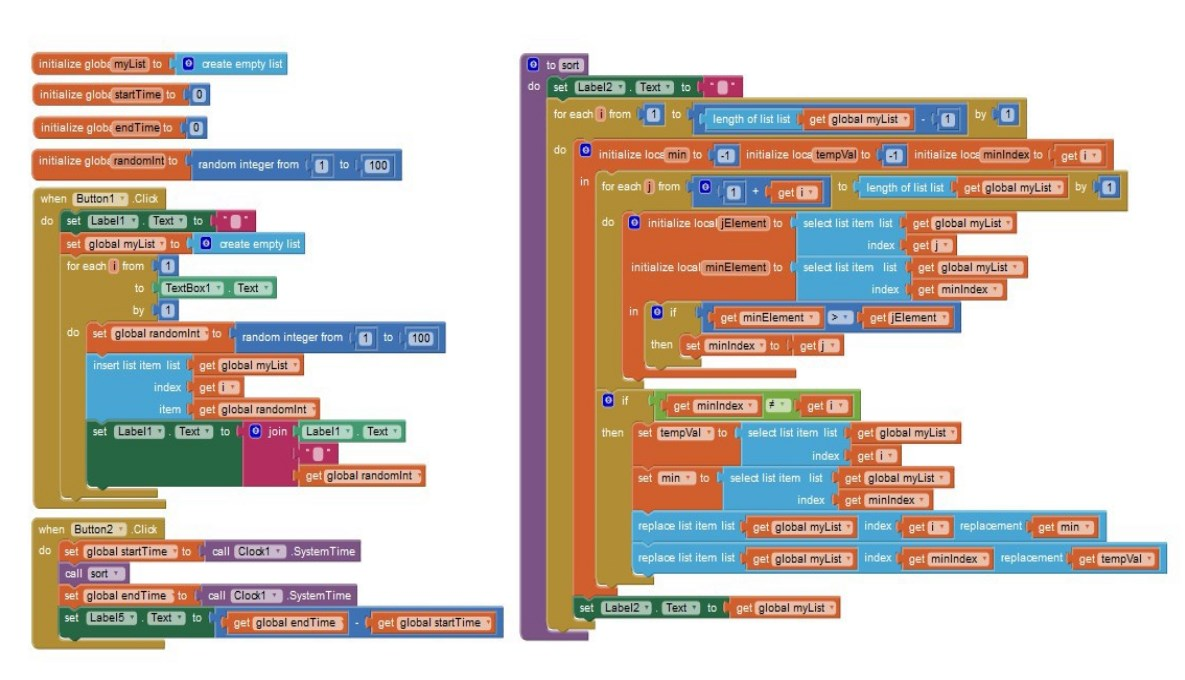
\includegraphics[width=15cm]{figures/apps/sort}
\caption{Aplikacja sortująca - App Inventor}
\end{figure}

Na powyższym rysunku widać bloki potrzebne do stworzenia aplikacji w App Inventorze. Bez głębszej analizy zrozumienie działania bloków, może okazać się kłopotliwe. Jest to prosty algorytm, a napisanie go za pomocą dostępnych bloków okazało się skomplikowane. Można sobie łatwo wyobrazić, że napisanie bardziej skomplikowanego algorytmu byłoby bardzo nieczytelne. Ilość użytych bloków zdecydowanie by wzrosła, dodatkowo utrzymanie takiej aplikacji niesie za sobą wysokie koszty wprowadzenia nowych osób do jej rozwijania.

Sortowanie napisanie w Javie jest zrozumiałe dla każdego programisty. Do sortowania została użyta lista, jako odpowiednik listy w App Inventorze, nie ma tam dostępnych tablic.


\begin{lstlisting}
 void sort(List<Integer> list){
        for(int i =0;i<list.size()-1;i++){
            int index = i;
            for(int j=i+1;j<list.size();j++){
                if(list.get(j) < list.get(index) ){
                    index = j;
                }
            }
            if(index != i){
                int tmp = list.get(i);
                list.set(i,list.get(index));
                list.set(index,tmp);
            }
        }
    }
\end{lstlisting}

W algorytmach bardzo ważna jest wydajność. Oba algorytmy działają w ten sam sposób, jednak wydajność sortowania listy napisanej w Javie jest zdecydowanie wyższa. Można to zaobserwować na poniższym wykresie. Przesortowanie bardzo małej liczby elementów zajmuje App Inventorowi bardzo dużo czasu. Przy 25 elementach czas sortowania przekroczył 1 sekundę. Jest to bardzo słaby wynik w porównaniu do sortowania napisanego w Javie. Średnio czas sortowania był 2 tysiące razy mniejszy! Na poniższym uwidaczniającym różnicę wykresie zastosowano skalę logarytmiczną, aby zobaczyć różnicę.

\begin{figure}[htbp]
\centering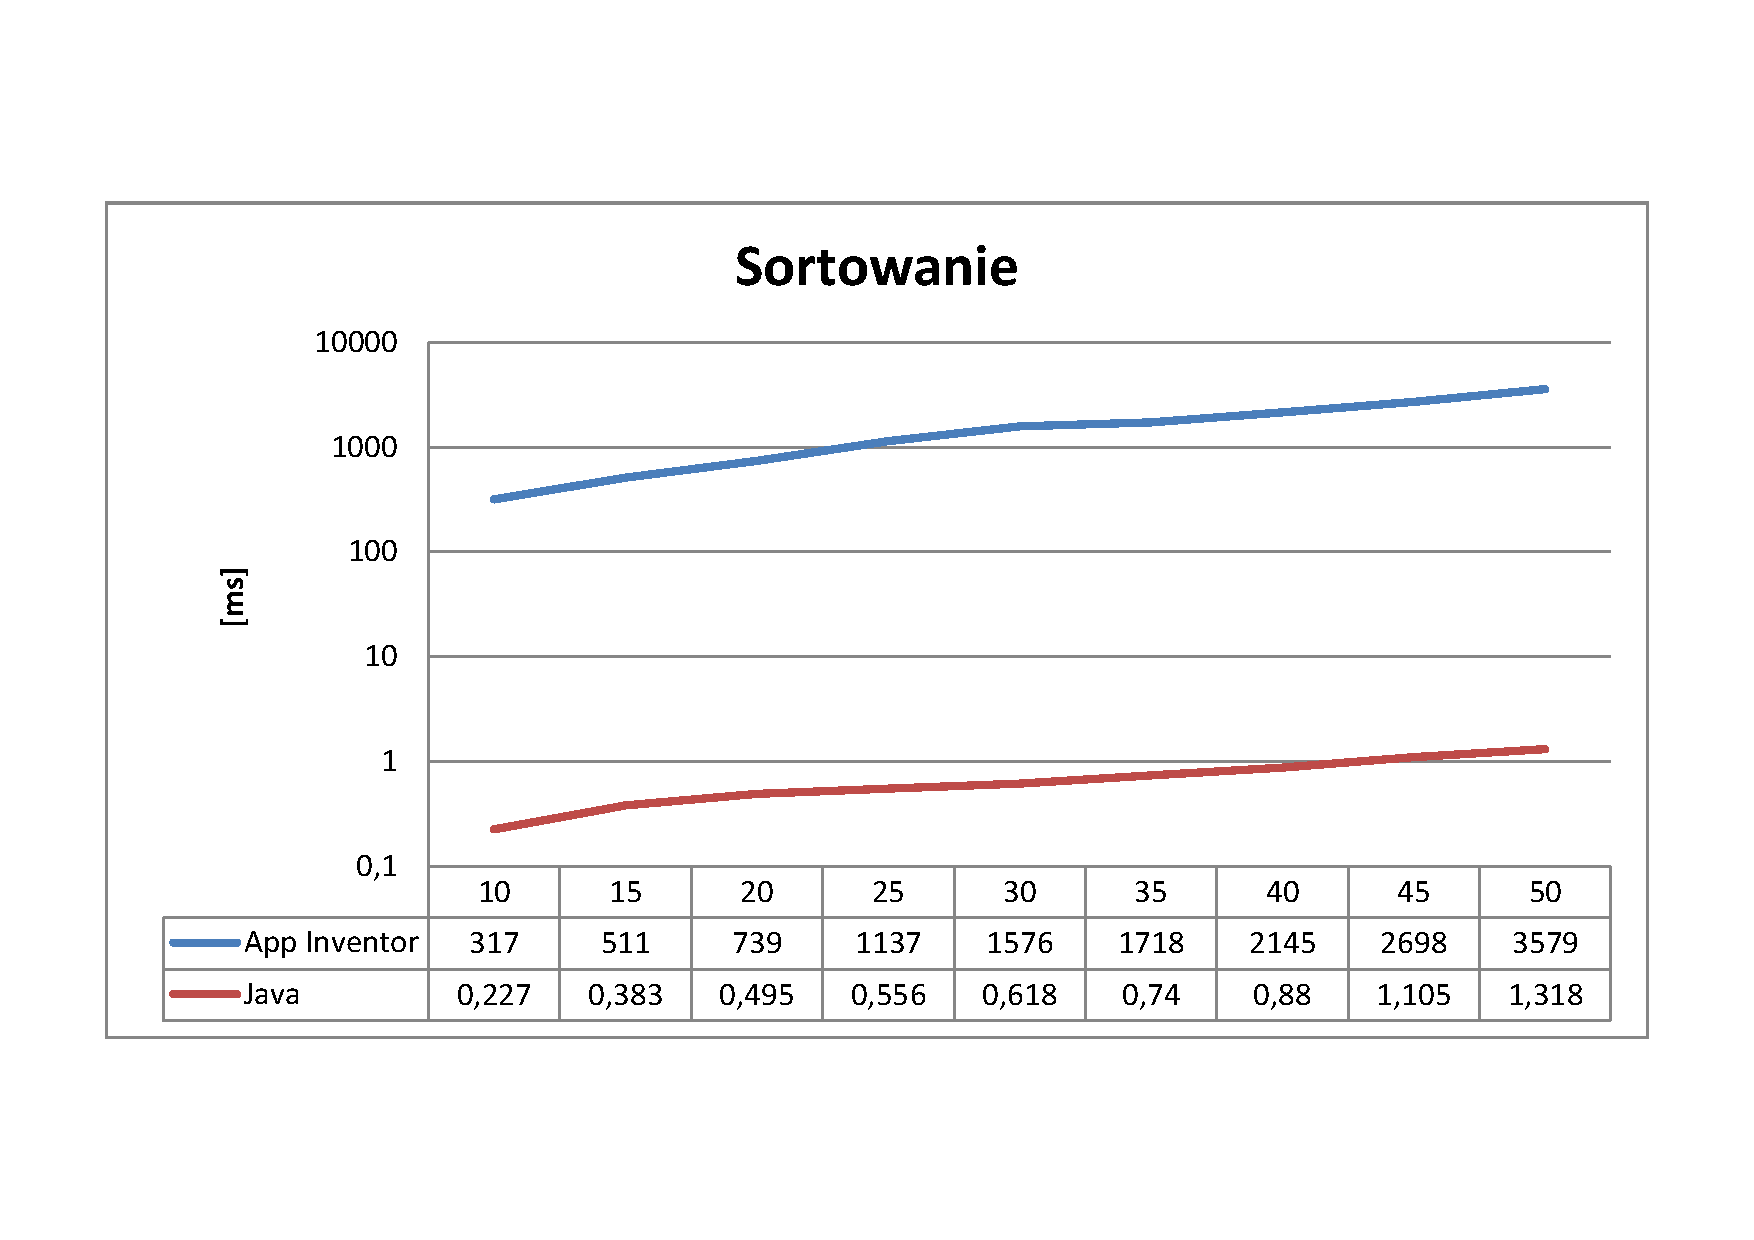
\includegraphics[width=10cm]{figures/apps/sortChart}
\caption{Wykres przedstawiający czas sortowania}
\end{figure}

Napisanie omawianej aplikacji w Javie nie było żadnym problemem. Bardzo łatwo było zdebugowano kod i sprawdzono jego poprawność. Stworzenie tej samej aplikacji w App Inventorze nie było trywialne.


\subsection{Fibonacci}

Następną stworzoną aplikacją jest aplikacja wyliczająca kolejny element ciągu Fibonnaciego. Testuje ona wydajność App Inventora. Złożoność takiego algorytmu to $O(2^n)$, czyli czas wykonywania będzie rósł bardzo szybko. Dodatkowo, kod jest napisany w taki sposób, aby metody wykonywały się rekurencyjnie, jednak aplikacja nie jest w stanie przetestować wielkości stosu. Dla bardzo małych liczb czas wykonywania się algorytmu jest bardzo wysoki.

\begin{figure}[H]
\centering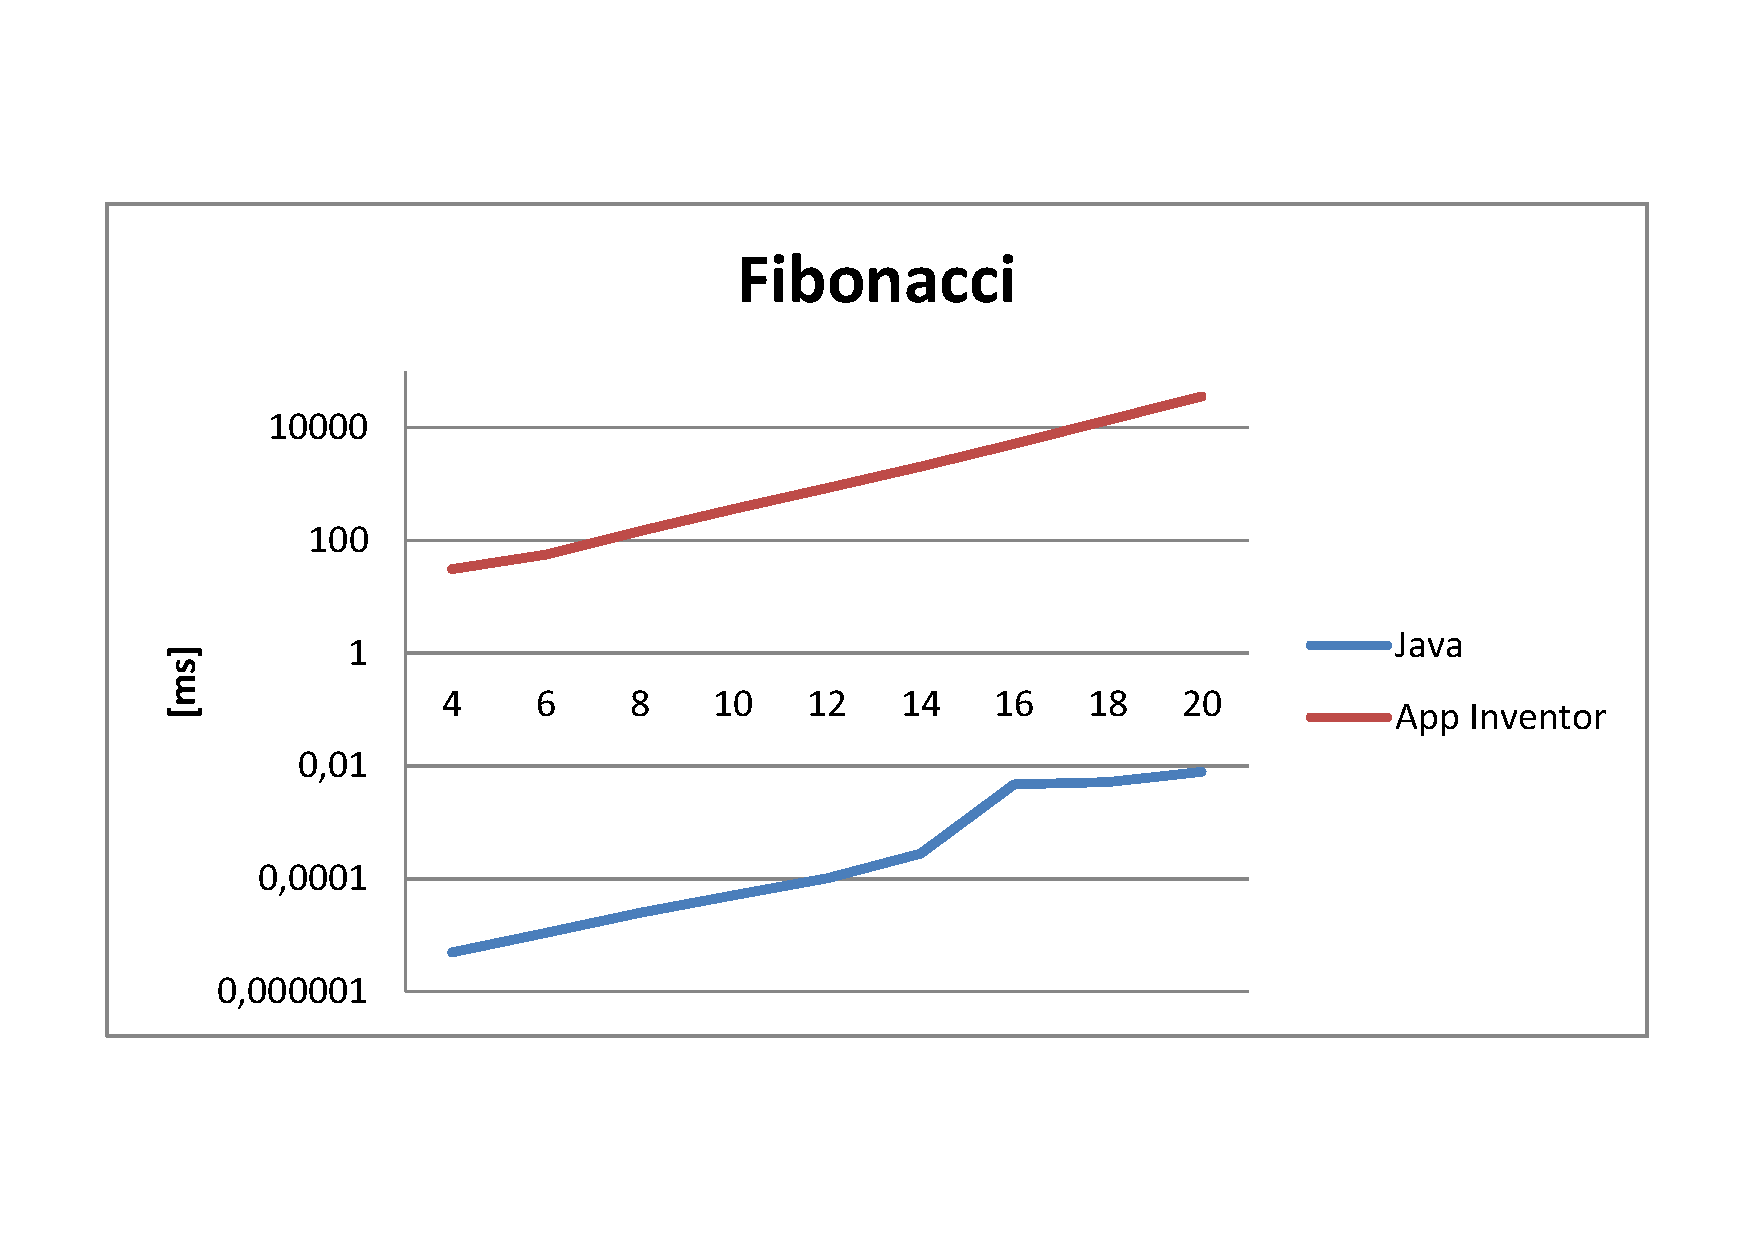
\includegraphics[width=10cm]{figures/apps/fibonacciChart}
\caption{Wykres przedstawiający czas obliczenia n-tego elementu z ciągu Fibonacciego}
\end{figure}

Osiągnięty rezultat wydajności nie jest zaskakujący po otrzymaniu wyników z poprzednich programów. Czas obliczenia już początkowych elementów ciągu Fibonnaciego jest bardzo duży. Przy liczeniu dwudziestego elementu aplikacja napisana w App Inventorze potrzebuje ponad pół minuty, podczas gdy, aplikacja napisana w Javie potrzebuje na to około jedną setną sekundy.


\subsection{Silnia}

Następny program oblicza silnię danego elementu. Istnieje możliwość wyboru, iteracyjna lub rekursyjna wersja. Aby zaprezentować oba podejścia na jednym wykresie, zastosowano skalę logarytmiczną.

\begin{figure}[H]
\centering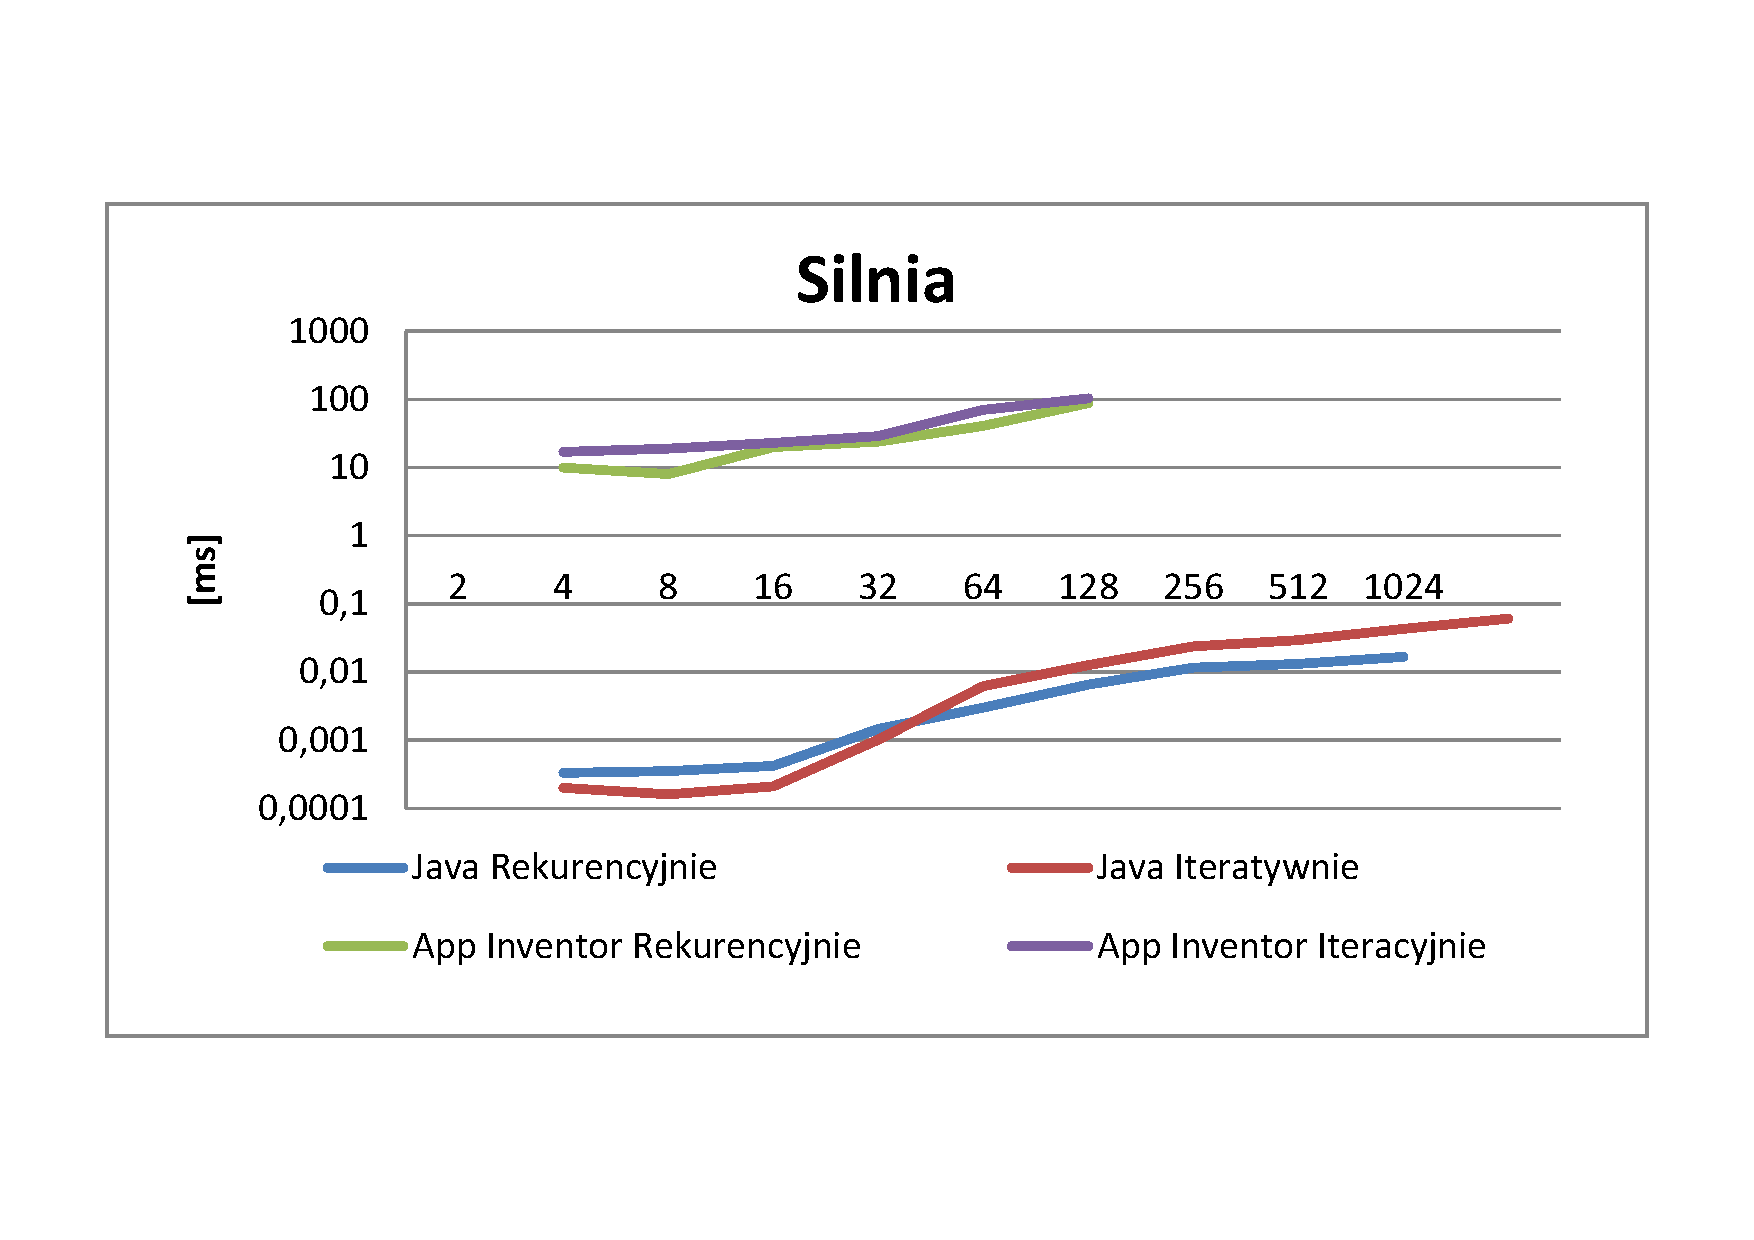
\includegraphics[width=10cm]{figures/apps/factorialChart}
\caption{Wykres przedstawiający czas obliczenia silni danego elementu}
\end{figure}

Na powyższym wykresie można zaobserwować wiele istotnych elementów. Aplikacja napisana w języku Java nie miała żadnych problemów w podejściu iteracyjnym. Zakres liczb nie został przekroczony, ze względu na możliwość wyboru typu danych. Potrzebna była tutaj klasa dla wielkich liczb całkowitych, dlatego został użyty typ BigInteger. Podczas użycia wersji rekurencyjnej, przy około liczeniu silni dla około 700, program rzuca wyjątek przepełnienia stosu (\english{Stack overflow}).

App Inventor umożliwia pisanie funkcji, a następnie wywołanie ich rekurencyjnie. Wygląda to w następujący sposób:

\begin{figure}[H]
\centering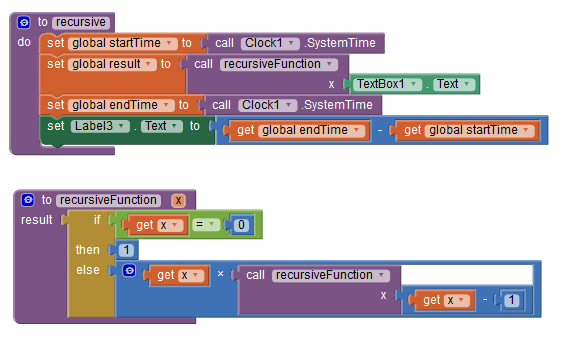
\includegraphics[width=10cm]{figures/apps/recursiveFunction}
\caption{Funkcja obliczająca silnie rekursywnie}
\end{figure}

Ciekawa sytuacja występuje dla aplikacji napisanej w App Inventorze. Program rzuca wyjątek podczas działania programu (\english{Runtime error}). Niestety, nie wiadomo co to za błąd, ponieważ w logach wiadomość o błędzie jest niedostępna. Wiadomość, którą otrzymujemy w logach wygląda następująco:

\begin{lstlisting}
E/com.google.appinventor.components.runtime.util.RuntimeErrorAlert:
No error message available
\end{lstlisting}

Można się jedynie domyślać, że jest to błąd przepełnienia stosu lub przekroczenia zakresu liczb.

\section{Aplikacje testujące wbudowane elementy telefonu}

\subsection{Akcelerometr}

Kolejną aplikacją jest wykorzystująca akcelerometr. Odczytuje ona dane z akcelerometru, a następnie wyświetla je na ekran telefonu, z zadaną częstotliwością. Na poniższym wykresie przedstawione jest zużycie procesora dla różnych wartości próbkowania. Można zauważyć, że zużycie procesora dla aplikacji napisanej w Javie jest prawie stałe. Dzieje się tak dlatego, że ustawianie częstotliwości próbkowania jest tylko wskazówką dla systemu. Zdarzenia mogą być odbierane szybciej lub wolniej niż zadana częstotliwość. Zazwyczaj są odbierane szybciej. W tym przypadku są odbierane szybciej i zmiana częstotliwości na mniejszą, tak naprawdę nic tutaj nie zmienia, ponieważ zdarzenia dalej będą odbierane szybciej. Zużycie procesora prawdopodobnie będzie dalej stałe, gdy będziemy zmniejszać częstotliwość.\cite{doc:android}

\begin{figure}[H]
\centering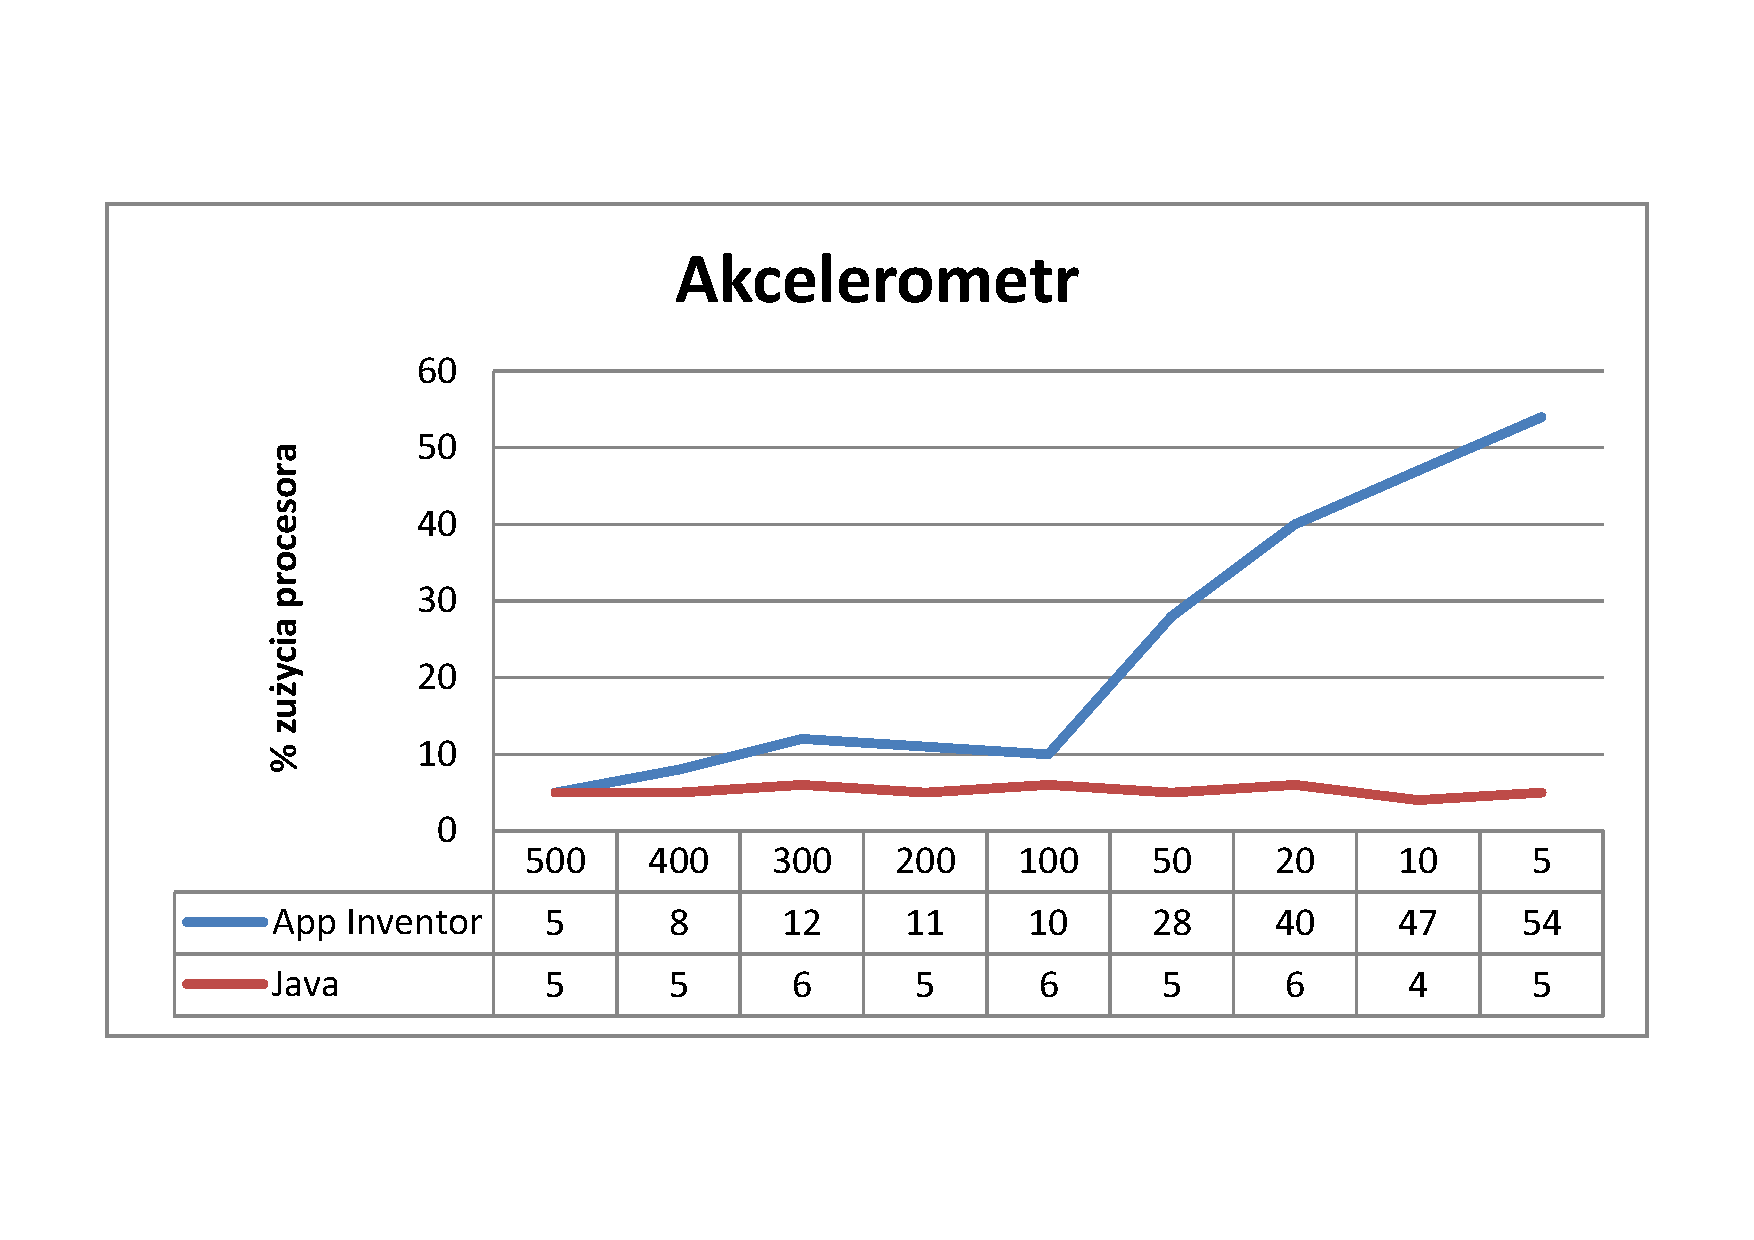
\includegraphics[width=10cm]{figures/apps/accelerometerChart}
\caption{Wykres przedstawiający zużycie procesora}
\end{figure}

W AppInventorze nie można zadać bezpośrednio akcelerometrowi częstotliwości próbkowania. Aby to obejść, trzeba dodać nowy komponent Clock, który ma możliwość uruchamiania, co zadany czas. Można podejrzewać, że wydajność akcelerometru jest niezmienna i częstotliwość próbkowania jest stała. Wyraźny spadek wydajności jest przez to, że musimy wywoływać metody w bardzo krótkich odstępach czasu i to, że one dodatkowo odczytują wartość sensora, nie wpływa znacząco na zużycie procesora.


\begin{figure}[H]
\centering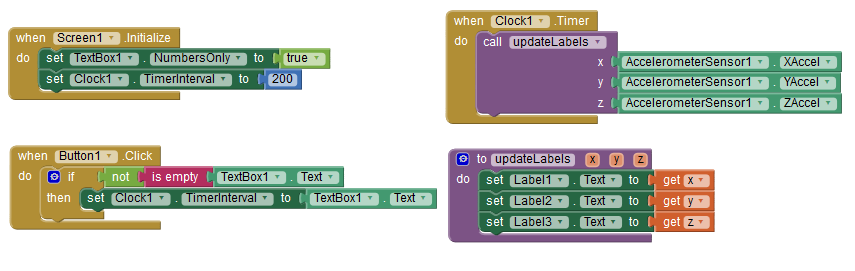
\includegraphics[width=14cm]{figures/apps/akcelerometerAI}
\caption{Bloki aplikacji z akcelerometrem}
\end{figure}

Powyżej zaprezentowane są bloki konieczne do stworzenia aplikacji z akcelerometrem. Jak widać jest to tylko kilka bloków. W Javie natomiast jest więcej rzeczy do wykonania i jeżeli nie mieliśmy styczności z danym komponentem trzeba przeczytać dokumentację. Główne rzeczy jakie należy zrobić to zaimplementować odpowiedni interfejs i zainicjować sensor przy uruchamianiu aplikacji.




\subsection{Database}

Aplikację stworzono celem kontroli szybkości działania bazy danych oferowanej przez App Inventora. Został tutaj wykorzystany komponent TinyDB. Odpowiada on klasie Javy SharedPreferences, czyli jest to baza danych typu klucz/wartość. Aby odczytać dane z pamięci trzeba znać klucz do tych danych. Jest to bardzo łatwe w przypadku małych ilości danych, jednak trudno jest przechowywać większy struktury, ze względu na potrzebę znania klucza dla każdego wiersza. Duże ilości danych powinny być przechowywane w bazie danych SQLite, ponieważ organizacja danych i zarządzanie nimi jest wydajniejsze. Aby otrzymać część danych z bazy, trzeba posłużyć się językiem zapytań SQL. Daje to możliwość wyszukiwania interesujących nas danych. Z drugiej strony zarządzanie i przeszukiwanie dużych zbiorów danych wpływa na wydajność, więc czytanie danych z bazy danych może być wolniejsze niż czytanie danych z SharedPreferences.

\begin{figure}[H]
\centering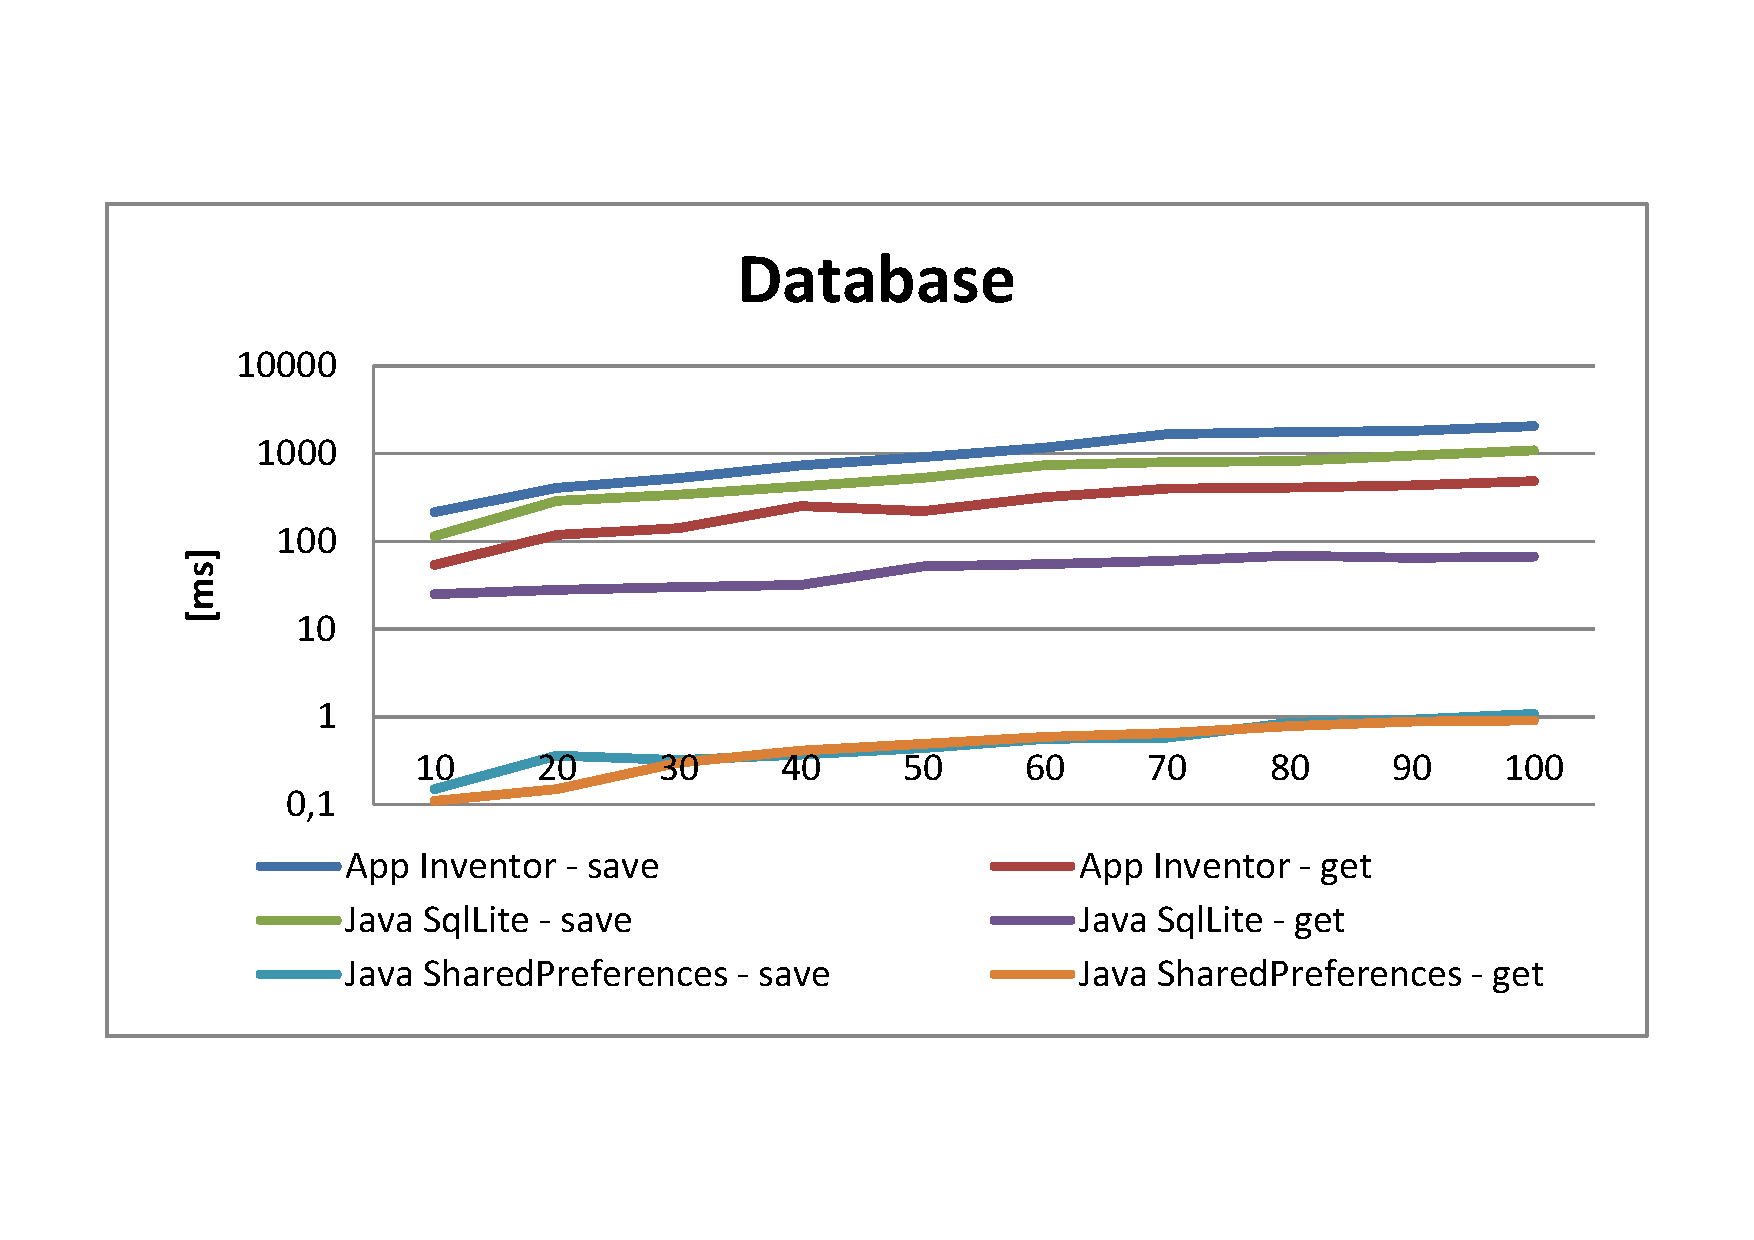
\includegraphics[width=10cm]{figures/apps/databaseChart}
\caption{Wykres przedstawiający czas potrzebny na zapis/odczyt n-elementów}
\end{figure}

Na powyższym wykresie można zauważyć przewagę wydajności aplikacji napisanej w Javie. App Inventor uzyskał podobny rezultat wydajności, jak aplikacja napisana w Javie, która używa bazy danych SQLite. Jak wspomniano wcześniej odczyt/zapis danych z bazy SQLlite powinien być wolniejszy niż korzystanie z SharedPreferences. SQLite uzykuje tutaj lepszy rezultat TinyDB - odpowiednik SharedPreferences. Można łatwo wyciągnąć wniosek, że wydajność TinyDB jest bardzo niska. Jeżeli porównamy TinyDB i SharedPreferences przewaga aplikacji napisanej w Javie jest ogromna.


\subsection{Animacja}

Aplikacja testuje możliwości animacyjne App Inventora. Wiadomo, że komponenty potrzebne są dostępne, jednak nie wiadomo, czy wydajność pozwoli na płynną animację. Mimo że tworzenie animacji może wydawać się trudne, za pomocą App Inventora stworzenie animacji odbywa się tylko w kilku krokach. Największym problemem było znalezienie odpowiednich klatek, gdzie ostatnia wygląda tak samo jak pierwsza, aby uzyskać możliwość zapętlenia.


\begin{figure}[H]
\centering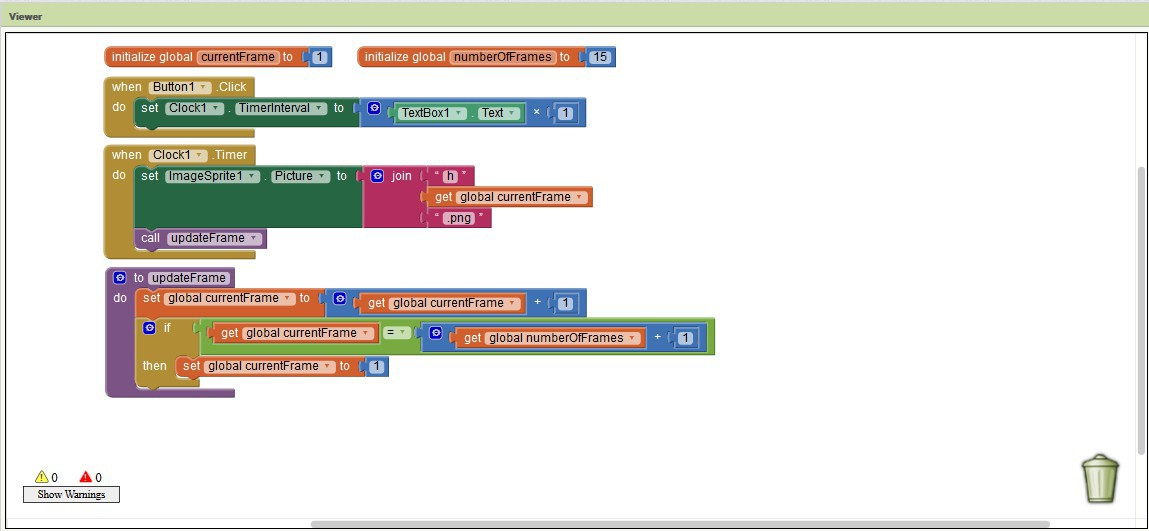
\includegraphics[width=15cm]{figures/apps/ai_animation}
\caption{Bloki potrzebne do stworzenia aplikacji}
\end{figure}

Na głównym ekranie aplikacji stworzone jest płótno oraz jeden obrazek, który podmieniamy co zadany interwał czasu. Ostatecznym rezultatem jest płynna animacja. Dopiero przy bardzo niskim interwale czasowym (szybkiej zmianie klatek), można było odczuć przycinanie się ekranu.


\subsection{Kolizja elementów}

Aplikacja sprawdzająca możliwość detekcji kolizji poruszających się elementów. Na płótnie umieszczono kilka elementów. Elementy w kolorze czarnym poruszają się po płótnie i kiedy dotrą do ściany odbijają się od niej. Element o kolorze niebieskim jest sterowanym za pomocą akcelerometru. Pochylając telefon przesuwamy element po płaszczyźnie.

\begin{figure}[H]
\centering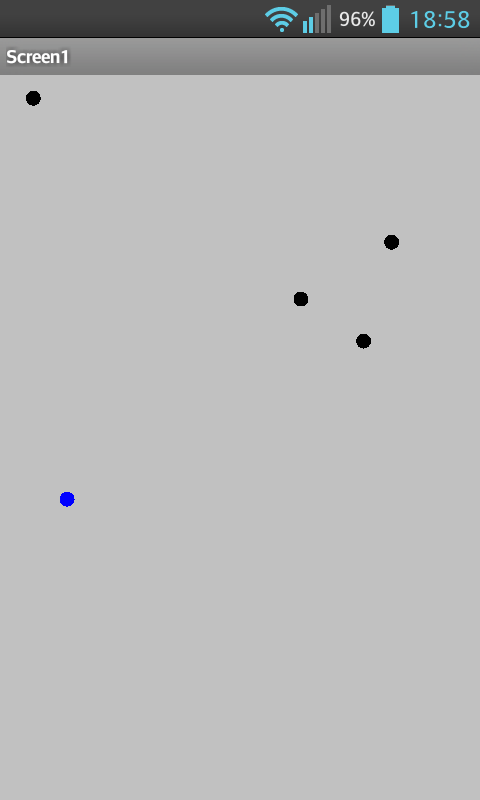
\includegraphics[width=5cm]{figures/apps/ai_collision}
\caption{Wygląd aplikacji testującej kolizje}
\end{figure}

Aplikacja działa płynnie, dla takiej ilości elementów. Wadą, którą można tutaj zauważyć, jest brak ogólnego komponentu odpowiedzialnego za zdarzenia lub możliwość przekazania parametru do zdarzenia. Jak widać na poniższym obrazku, tyle ile mamy komponentów, tyle musimy stworzyć zdarzeń odpowiedzialnych za odbicie od ściany. W danym przypadku nie jest to większym problemem. Ale kiedy istnieje potrzeba stworzenia aplikacji, która ma tych komponentów znaczącą ilość, jedną opcją jest wyklikanie zdarzeń po kolei dla wszystkich elementów.


\begin{figure}[H]
\centering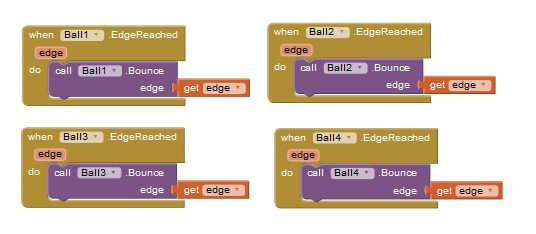
\includegraphics[width=10cm]{figures/apps/ai_collision_blocks}
\caption{Bloki odpowiedzialne za zdarzenia kolizji ze ścianą}
\end{figure}

\subsection{Activity Starter}

Aplikacja daje możliwość wystartowania nowego Activity, w App Inventor istnieje sposobność stworzenia jednej aplikacji, która będzie uruchamiała pozostałe. Odpowiedzialny za to jest komponent ActivityStarter. Wystarczy ustawić mu dwie właściwości, nazwę pakietu oraz klasy. Jeżeli w dokumentacji aplikacji nie napisano jakie są powyższe nazwy, warto uruchomić aplikację z podłączonym urządzeniem do komputera, aby widzieć logi. Należy wówczas znaleźć wtedy linijkę podobną do poniższej

\begin{lstlisting}
I/ActivityManager:
START {act=android.intent.action.MAIN cat=[android.intent.category.LAUNCHER]
flg=0x10200000 cmp=org.mozilla.firefox/.App u=0} from pid 726
\end{lstlisting}

Jeżeli pojawi się fragment z parametrem cmp, to nazwą pakietu jest tekst przed ukośnikiem, a nazwą klasy jest cały tekst bez ukośnika. Zatem komponent ActivityStarter daje możliwość uruchomienia prawie każdej aplikacji. Aplikacja nie musi być stworzona w App Inventorze, może to być dowolna aplikacja zainstalowana na urządzeniu. Istnieje również możliwość przekazania dodatkowych parametrów, przy uruchamianiu zewnętrznej aplikacji. Niektóre z nich są nawet zaprojektowane w ten sposób, aby przyjmować dodatkowe parametry podczas uruchamiania. Przykładem są tutaj aplikacja map, która przyjmie jako parametr wartości geograficzne. Innym przykładem jest wyszukiwarka internetowa, która przyjmie jako parametr tekst do wyszukania lub adres do wyświetlenia.

\begin{lstlisting}
Action: android.intent.action.VIEW
DataUri: http://google.pl
\end{lstlisting}

Ustawiając powyższe parametry, uruchomi się przeglądarka internetowa na stronie http://google.pl. Druga możliwość, jaką daje ActivityStarter, to odbieranie parametrów. W App Inventorze istnieje tylko przekazywanie wartości tekstowych. Aby zwrócić taki parametr trzeba użyć bloku zamykającego aplikację z właściwością do ustawienia (\english{Close Application With Plain Text}).

\subsection{Multiple Screens}

Jeżeli obie aplikacje mają być napisane przez tego samego programistę, warto się zastanowić, czy nie zrobić jednej aplikacji z wieloma ekranami. Zwiększy to użyteczność aplikacji, użytkownicy nie będą musieli instalować dwóch. Używając ActivityStartera dotychczas istnieje możliwość przekazywania tylko parametrów tekstowych. Natomiast przy użyciu wielu ekranów, można przekazywać dodatkowo listy. Kiedy aplikacja korzysta z bazy danych, również jest ona współdzielona pomiędzy ekranami. Otworzony ekran daje możliwość powrotu do ekranu, który go otworzył. Ilość ekranów nie jest ograniczona, ale zamknięcie ekranu powraca do tego, który go otworzył. Z drugiej strony łatwo to obejść, tworząc ekran, który będzie menadżerem innych ekranów i będzie on uruchamiał pozostałe. Jeżeli z uruchomionego ekranu użytkownik będzie chciał przejść do innego, aplikacja powróci do menadżera z parametrem, a menadżer w odpowiedzi na dany parametr otworzy inny ekran. Zatem tak samo jak w przypadku aplikacji wykorzystującej komponent ActivityStarter istnieje możliwość przekazywania i odbierania parametrów pomiędzy ekranami. Każdy stworzony ekran będzie miał swój wygląd oraz własne komponenty w oknie Designera. Stworzenie jednej bazy danych może być trochę nieintuicyjnie, ponieważ każdy ekran musi posiadać swój komponent TinyDB. Aczkolwiek jest to jedna i ta sama baza danych. Jeżeli jeden ekran zapisze jakąś wartość, drugi może ją od razu odczytać.

\subsection{Usługa POST/GET}

Aplikacja została stworzona aby przetestować komponent umożliwiający wysyłanie żądań typu GET i POST. Jako serwis obsługujący dane żądania został wybrany produkt Google o nazwie Google Charts.\cite{android:56} Jest to usługa tworząca wykresy poprzez zdefiniowanie odpowiedniego linku. Zazwyczaj są to żądania restowe, czyli za pomocą metody GET. Jednak liczba znaków w linku jest ograniczona do 2 tysięcy, dlatego czasem, trzeba skorzystać z metody POST. 


\begin{figure}[H]
\centering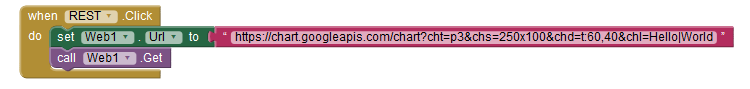
\includegraphics[height=2cm]{figures/apps/getRequest}
\caption{Bloki tworzące żądanie typu GET}
\end{figure}

\begin{figure}[H]
\centering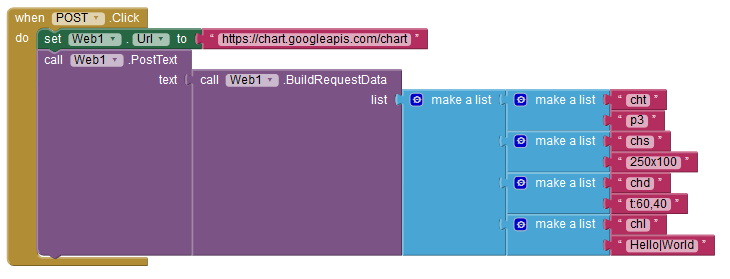
\includegraphics[height=6cm]{figures/apps/postRequest}
\caption{Bloki tworzące żądanie typu POST}
\end{figure}

Powyżej zaprezentowane są bloki potrzebne do stworzenia obu żądań. Przed wysłaniem żądania należy jest ustawić flagę zapisu plików na kartę SD na \emph{TRUE}. Inaczej nie wywoła się zdarzenie otrzymania pliku z serwera. Jak widać obsługa żądań typu GET jest bardzo prosta. Programista musi podać cały link, a następnie przypisać obrazkowi odebrany plik. Przy żądaniu typu POST, do funkcji trzeba przekazać parametry w inny sposób. Mianowicie trzeba stworzyć listę, która składa się z list 2 elementowych zawierających dane w formacie klucz, wartość.


\begin{figure}[H]
\centering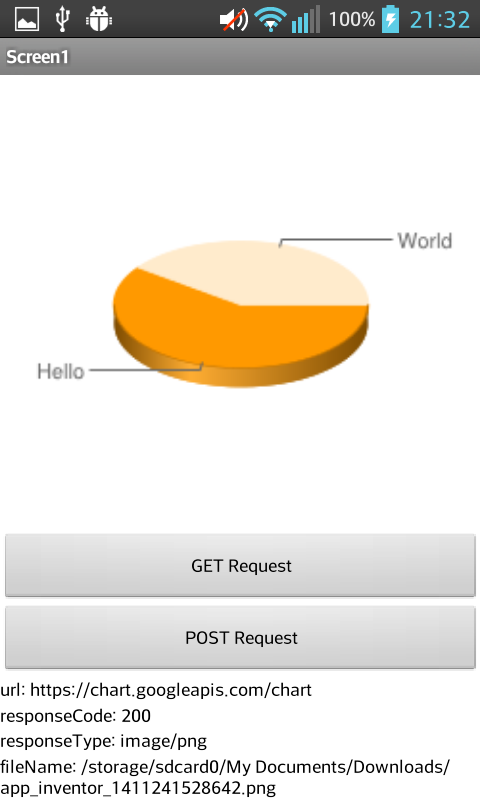
\includegraphics[height=10cm]{figures/apps/googleChart}
\caption{Aplikacja obsługująca żądania POST i GET}
\end{figure}

Na powyższym rysunku przedstawiona jest graficzny wygląd aplikacji. Posiada ona 2 przyciski, pod którymi znajdują się 2 różne żądania. Powyżej przycisków znajduje się obrazek, który jest wypełniany w momencie otrzymania odpowiedzi z serwera. Poniżej znajdują się parametry odpowiedzi.

\subsection{Import/Eksport danych z/do pliku CSV}

Aplikacja daje możliwość wyboru kontaktów za pomocą komponentu Contact Picker. Kontakty zapisuje do listy. Następnie ta lista jest konwertowana i zapisywana do pliku csv.

\begin{figure}[H]
\centering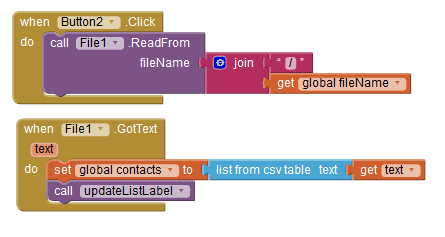
\includegraphics[height=5cm]{figures/import}
\caption{Bloki odpowiadające za import danych z pliku}
\end{figure}

\begin{figure}[H]
\centering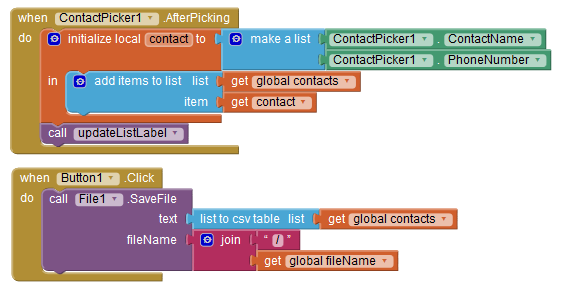
\includegraphics[height=5cm]{figures/export}
\caption{Bloki odpowiadające za eksport danych}
\end{figure}

Aplikacja działa bez zarzutu. Jedynym problemem była nazwa pliku, którą musi poprzedzać ukośnik. Wtedy dopiero App Inventor odczytuje plik z karty pamięci. Jeżeli nazwę pliku poprzedzają 2 ukośniki App Inventor szuka pliku w swoich assetach. Jeżeli nazwy pliku nie poprzedza żaden ukośnik, znajduje się on w prywatnej bazie App Inventora.

Eksport kontaktów był okazał się bezproblemowy. Eksportowana lista zawierająca inne listy odpowiada tabeli. Każdy wiersz tabeli jest wewnętrzną listą. Podczas importu dane mają taką samą strukturę.

\section{Odtworzenie aplikacji napisanej w Javie}

\subsection{Think Faster}

App Inventor oferuje bardzo wiele elementów i rozwiązań. Celem sprawdzenia, jak zachowują się one w praktyce podjęto próbę skopiowania gry napisanej wcześniej w języku Java. Jest to gra o nazwie \emph{Think Faster}. Znajduje się ona w markecie Google Play pod poniższym adresem internetowym:

\begin{lstlisting}
https://play.google.com/store/apps/details?id=com.thinkfaster
\end{lstlisting} 

Gra polega na rozwiązywaniu działań matematycznych o różnym stopniu trudności. 

\begin{figure}[H]
\centering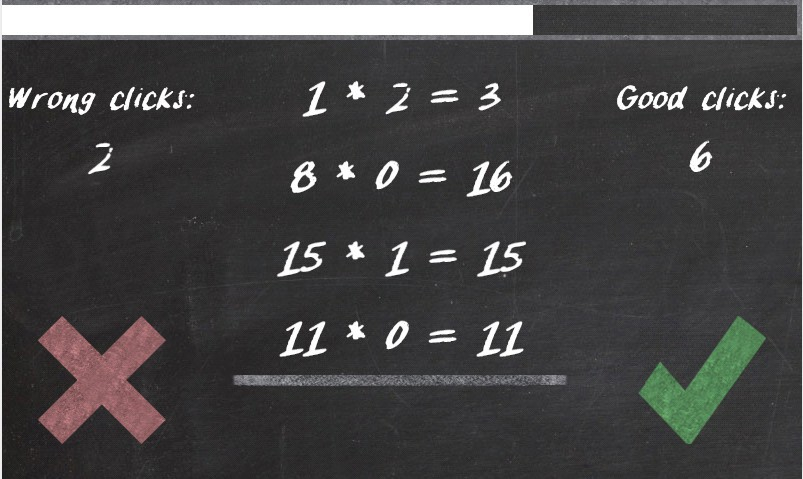
\includegraphics[width=10cm]{figures/apps/thinkfaster_newgame}
\caption{Główny ekran aplikacji}
\end{figure}

Na powyższym ekranie widać w jaki sposób użytkownik musi rozwiązywać działania matematyczne. Do rozwiązania jest ostatnie działanie na dole ekranu. Można zauważyć, że jest ono błędne, więc gracz powinien kliknąć krzyżyk. Działania będą płynnie przesuwały się z góry na dół. Po nabraniu wprawy, można patrzeć na więcej przykładów, niż tylko to na samym dole i tym samym szybciej je rozwiązywać, co skutkuje większą ilością punktów. Na górze ekranu widać uciekający czas. Po prawidłowym kliknięciu czas zostaje minimalnie zwiększony oraz przez chwilę robi się zielony. Odwrotnie jest przy nieprawidłowym rozwiązaniu przykładu i kliknięciu nie tego przycisku. Część czasu zostaje ucięta i zabarwiona na chwilę na czerwono. Do napisania tej gry użyto dodatkowo bibliotekę AndEngine, która umożliwia animację dwuwymiarową i znacznie ułatwia pisanie kodu.


\begin{figure}[H]
\centering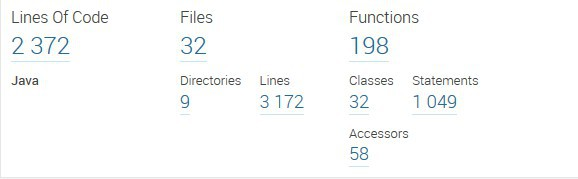
\includegraphics[width=10cm]{figures/sonarThinkFaster}
\caption{Statystyki zebrane przez aplikację Sonar}
\end{figure}

Można wywnioskować zatem z powyższego opisu oraz ze statystyk przedstawionych przez aplikację Sonar, że \emph{Think Faster} nie jest bardzo skomplikowaną grą. Około dwa tysiące linii kodu, z czego część jest testami, nie robi dużego wrażenia.

Próba skopiowania takiej aplikacji nie zakończyła się całkowitym sukcesem, ale nie można powiedzieć, że zakończyła się porażką.

Na samym początku tworzenia pojawił się problem z paskiem statusu androida, którego nie da się schować w App Inventorze. Mimo wszystko istnieje do tego obejście. Trzeba pobrać plik \emph{apk} na komputer. Następnie go zdekompilować i wyedytować plik \emph{AndroidManifest.xml} dodając następującą właściwość, w każdym Activity, w którym nie ma się pojawiać pasek statusu:
\begin{lstlisting}
android:theme="@android:style/Theme.NoTitleBar.Fullscreen"
\end{lstlisting}
Aplikację następnie trzeba zbudować i podpisać cyfrowo, aby zainstalować ją na urządzeniu.

Następnym problemem, jaki powstał, był problem optymalizacyjny. Aplikacja napisana w Javie podczas przełączania ekranów, ładowała do pamięci grafiki, wyświetlając przy tym napis \emph{Loading...}. Jest to niemożliwe do zrealizowania w App Inventorze. Jeżeli ekran posiada wiele elementów, a funkcja inicjalizująca ekran jest skomplikowana i czasochłonna, użytkownik może odnieść wrażenie, że urządzenie przestało odpowiadać. Podczas ładowania ekranów, dodatkowo użytkownikowi wyświetlały się reklamy, które są niemożliwe do stworzenia w App Inventorze.

Ekran menu w oryginalnej aplikacji wygląda następująco:

\begin{figure}[H]
\centering
\includegraphics[width=10cm]{figures/apps/thinkfaster_menu}
\caption{Ekran menu gry}
\end{figure}

Ekran nie jest skomplikowany. Dlatego też całkowicie udało się go odtworzyć w App Inventorze. Wykorzystano komponent Canvas, a poszczególne przyciski były obrazkami z danym napisem. Zaczynając od dołu ekranu, przycisk wyjście udało się obsłużyć i wyjść z aplikacji. Dodatkowo istnieje zdarzenie naciśnięcia klawisza systemowego wstecz, który można obsłużyć we własny sposób. Powiodła się również próba całkowitego odtworzenia ekranu pomocy. Zawiera on jedynie komponent Canvas rozciągnięty na cały ekran, na którym znajduje się obrazek.

Wybierając nową grę użytkownik przechodzi do wyboru ekranu z typem gry. Zaprezentowany ekran widać poniżej:

\begin{figure}[H]
\centering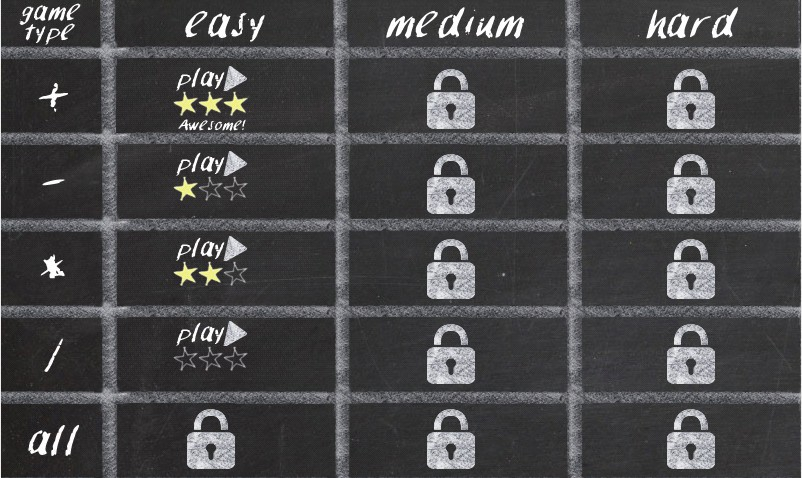
\includegraphics[width=10cm]{figures/apps/thinkfaster_gametype}
\caption{Ekran wyboru rodzaju gry}
\end{figure}

Na tym ekranie użytkownik wybiera poziom trudności oraz przykłady, jakie chciałby rozwiązywać. O ile taki ekran programista jest w stanie stworzyć używając komponentów App Inventora, o tyle wiele trudności przyniosłoby wtedy stworzenie głównego ekranu gry. Poniżej nastąpi uzasadnienie tego stwierdzenia.

Uruchamiając nową grę wiele rzeczy na początku musi zostać stworzone. Pierwszym z elementów jest pasek z uciekającym czasem. Został stworzony jako prostokątny obrazek przesuwający się w lewo. Jedynym problemem było, kiedy nastąpiła kolizja ze krawędzią ekranu. W App Inventorze nie ma możliwości wyłączenia jej. Obejście tego problemu to zmniejszanie rozmiaru obrazka z taką samą prędkością jaką poruszał się on na początku.

Kolejnym elementem są przyciski, mówiące przy działanie matematyczne jest poprawne lub niepoprawne. Przy tworzeniu ich nie pojawiły się żadne problemy. Są to zwykłe obrazki nałożone na płótnie. Posiadają one zdarzenie \emph{TouchUp}, które jest wywoływane w momencie podniesienia palca z przycisku.

Przy tworzeniu następnych elementów zaczynają się trudności. Możliwe jest dynamiczne stworzenie działań matematycznych i umieszczenie ich na etykietach. Jednak niemożliwe jest stworzenie tych działań i przeniesienie ich na obrazek na płótnie. W celu obejścia takiego problemu można wykorzystać możliwość wcześniejszego, ręcznego stworzenia wymaganych obrazków i załadowanie ich do pamięci telefonu. Aby uzyskać animację znowu pojawia się problem aby dynamicznie stworzyć nowy obrazek na nowy przykład matematyczny i usunąć ten rozwiązany. Rozwiązanie tego problemu to korzystanie tylko z 3-4 przykładów dostępnych na ekranie. Rozwiązanemu przykładowi ustawiamy widoczność na fałsz i przesuwamy do na górę ekranu, podczas gdy reszta elementów przesuwa się standardowo na dół.

Na ekranie są zamieszczone 2 liczniki pokazujące liczbę poprawnych i niepoprawnych kliknięć. Wydawać by się mogło, że są one proste do zaimplementowania. Otóż okazuje się że w App Inventorze bardzo trudno zrobić taki licznik, ponieważ ten licznik jest obrazkiem. Przy ładowaniu ekranu musimy wczytać wszystkie 10 cyfr i po kliknięciu taki nimi manipulować, aby stworzyć odpowiednią liczbę.

Podsumowując powyższe obserwacje należy stwierdzić, że największy problem stanowi dynamiczne ustawianie tekstu na obrazku. Niestety nie jest to możliwe w App Inventorze. Okazuje się jednak, że prawie każdy problem można w mniej lub bardziej pracochłonny sposób rozwiązać. Wniosek jaki można tutaj postawić to, że jeżeli będziemy chcieli tworzyć grę, posiadającą wiele animacji, to lepiej się zastanowić, czy nie skupić się na nauce programowania w Javie i poznaniu bibliotek wspomagających rysowanie grafiki dwuwymiarowej.

